Si alguna vez ha utilizado PHP o ASP, probablemente esté acostumbrado a la idea de que el servidor web (Apache o IIS, por ejemplo) sirve sus archivos estáticos para que un navegador puede verlos a través de la red. Node ofrece un paradigma diferente al de un servidor web tradicional: la aplicación es el servidor web. Node simplemente proporciona las bases para que se pueda construir un servidor web. 

\subsection{Servidor NodeJS}
El modelo de E/S impulsado por eventos sin bloqueo le brinda a NodeJS un rendimiento muy atractivo, superando fácilmente los entornos de servidores como PHP y Ruby on Rails, que bloquean las E/S y manejan múltiples usuarios simultáneos en hilos separados para cada uno. Algo importante que se debe saber es que NodeJS no es un \gls{framework} sino un entorno, hay \glspl{framework} que funcionan con Node, como Express y Sails, lo que facilita la creación de aplicaciones.
\vspace{0.8cm}

\begin{figure}[H]
  \centering
  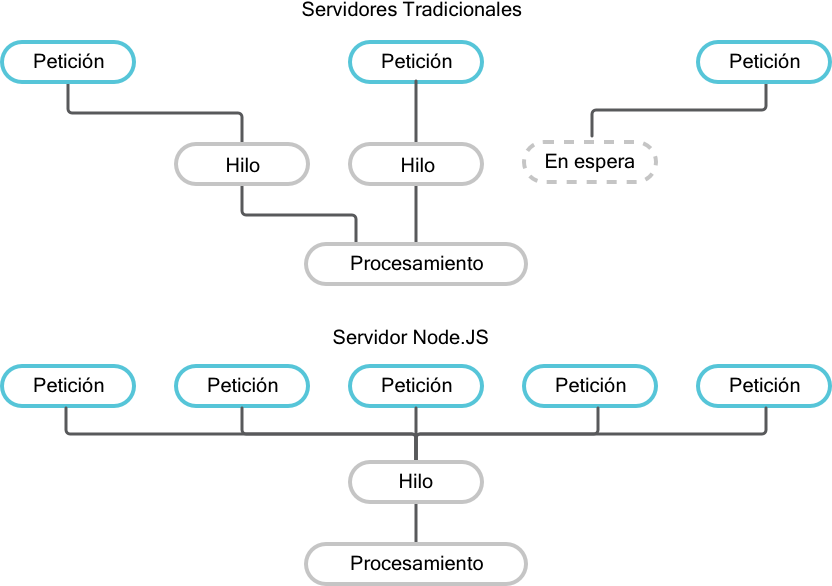
\includegraphics[width=0.8\textwidth]{node-traditional}
  \caption{Comparación de node y servidores tradicionales. (Fuente: Advance Idea Infotech 2018)}
\end{figure}

Un servidor Node.js tiene un solo subproceso de bucle de eventos (event-loop) que espera E/S en sockets y archivos. Una vez que los datos están listos, activa el método de evento correspondiente y espera hasta que regrese antes de esperar nuevamente por más eventos de E/S. Dado que todas las operaciones de E/S no bloquean, se asegurará de que todo se ejecute correctamente tan pronto como la entrada esté disponible sin ningún bloqueo y sin que se tenga lidiar con problemas de subprocesos múltiples.

\newpage
\subsubsection{Programación basada en eventos}
La filosofía central detrás de NodeJS es la programación basada en eventos. Significa que, el programador,  debe comprender qué eventos están disponibles y cómo responder a ellos. Muchas personas se introducen en la programación basada en eventos mediante la implementación de una interfaz de usuario: el usuario hace clic en algo y se dispara el `evento clic'. Es una buena metáfora, porque se entiende que el programador no tiene control sobre cuándo, o si el usuario va a hacer clic en algo, por lo que la programación basada en eventos es realmente bastante intuitiva \cite{ethan}.
\vspace{0.8cm}

\lstinputlisting[label={node-server}, style=ES6, caption=Configuración servidor NodeJS básico]{code/node-server.js}
En el ejemplo de código \ref{node-server}, el evento es implícito: el evento que se está manejando es una solicitud HTTP. El método http.createServer toma una función como argumento; esta función se invocará cada vez que se realice una solicitud HTTP. El programa simplemente establece el tipo de contenido en texto sin formato y envía la cadena `Hola, mundo!'.


\subsection{Configuración Express}
Express.js es un `marco de aplicación web NodeJS minimalista y flexible' \cite{express}. Es una capa delgada de características, fundamental para cualquier aplicación web, agrega tres características poderosas: enrutamiento, mejores manejadores de solicitudes y vistas.

\subsubsection{Enrutamiento}
Enrutamiento se refiere al mecanismo para servir al cliente el contenido que ha solicitado. Para las aplicaciones cliente/servidor basadas en web, el cliente especifica el contenido deseado en la URL (ruta y cadena de consulta).\\[0.8cm]
Cuando una aplicación Express.js se está ejecutando, escucha las solicitudes. Cada solicitud entrante se procesa de acuerdo con una cadena definida de middlewares y rutas que comienzan de arriba a abajo. Este aspecto es importante porque le permite controlar el flujo de ejecución \cite{azat}.
\vspace{0.8cm}

\begin{figure}[H]
  \centering
  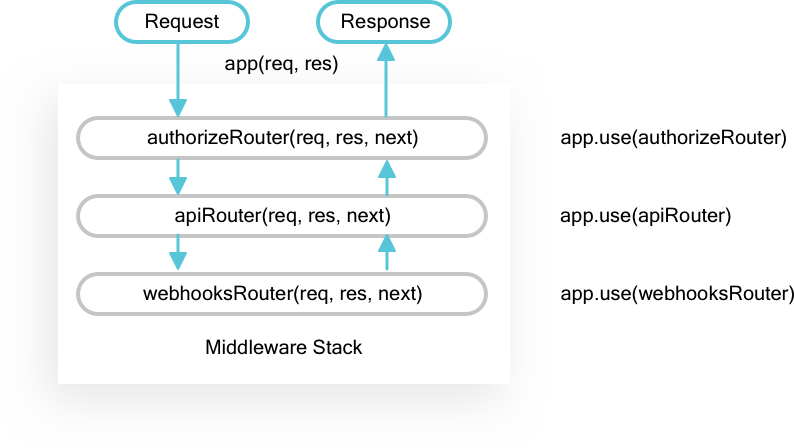
\includegraphics[width=0.8\textwidth]{express-router}
  \caption{Cada función de middleware en la pila se ejecuta antes que las que están debajo de ella. (Fuente: Elaboración propia)}
\end{figure}

\newpage
\lstinputlisting[style=ES6, caption=Fragmento de la configuración de enrutamiento del sistema]{code/express-router.js}

\subsection{Configuración Firebase}
Antes de conectar nuestro sistema con una base de datos de Firestore es necesario crear una aplicación en la consola de Google Firebase y seguir los siguientes pasos.
\vspace{0.8cm}

\begin{figure}[H]
  \centering
  
\includegraphics[width=1\textwidth]{firebase-01}
  \caption{Consola de Google Firebase. (Fuente: Google Console)}
\end{figure}

\begin{enumerate}
  \item Crear un nuevo proyecto en la consola de Firebase.

  \begin{figure}[H]
    \centering
    
\includegraphics[width=1\textwidth]{firebase-02}
  \end{figure}

  \item En el apartado `Database', seleccionar `crear base de datos' .

  \begin{figure}[H]
    \centering
    
\includegraphics[width=1\textwidth]{firebase-03}
  \end{figure}

  \item En la ventana emergente, seleccionar reglas de seguridad y definir ubicación del servidor.

  \begin{figure}[H]
    \centering
    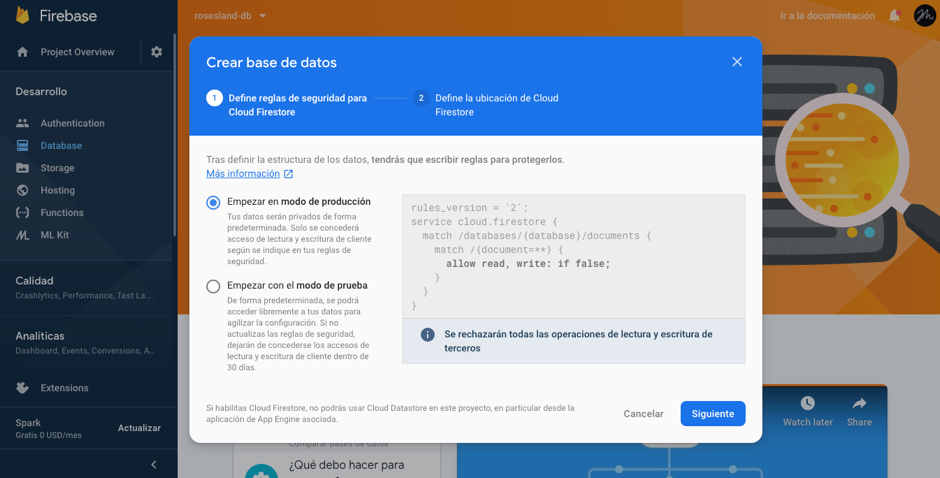
\includegraphics[width=1\textwidth]{firebase-04}
  \end{figure}

  \item El siguiente paso es generar las claves que permitan usar `firebase-admin' en el \gls{backend}. En la configuración del proyecto debajo del apartado `cuentas de servicio', presionar el botón `Generar cuentas de servicio'. El contenido del archivo JSON generado se debe de agregar a las variables del entorno que correspondan.

  \begin{figure}[H]
    \centering
    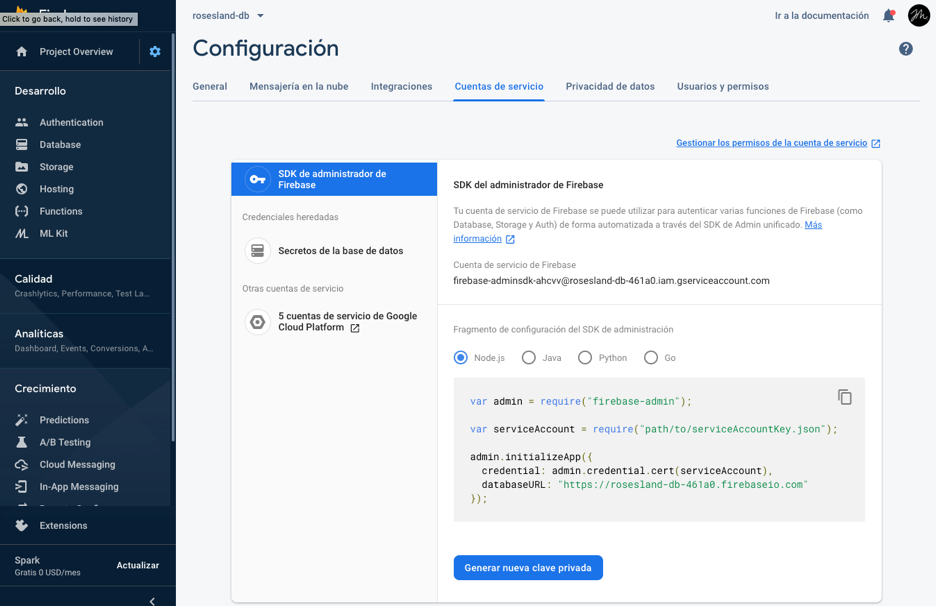
\includegraphics[width=1\textwidth]{firebase-05}
  \end{figure}

  \item Por ultimo en la sección `Authentication' se deben activar los servicios de autenticación necesarios, para este proyecto es necesario activar la validación por correo electrónico y contraseña.

  \begin{figure}[H]
    \centering
    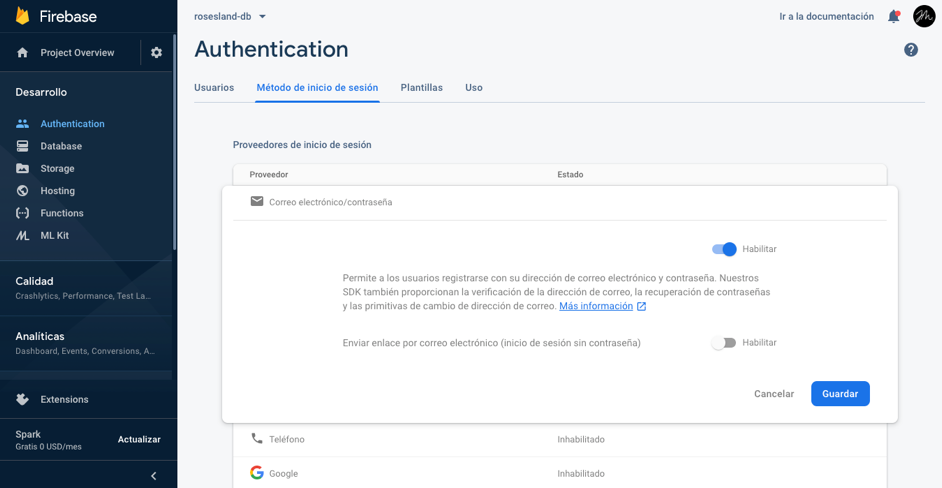
\includegraphics[width=1\textwidth]{firebase-06}
  \end{figure}
\end{enumerate}

\newpage
\subsubsection{Configuración de Firebase Firestore en Node.js}
Después de crear el objeto de configuración, es necesario inicializar Firebase en la aplicación de la siguiente manera:
\vspace{0.8cm}

\lstinputlisting[label={node-firebase}, style=ES6, caption=Fragmento de la configuración Firebase en el servidor]{code/firebase.js}

\subsubsection{Escrituras en lotes}
Para manipular documentos en un conjunto de operaciones, se pueden ejecutar varias operaciones de escritura como un lote único que incluya cualquier combinación de operaciones set(), update() o delete(). El lote de escrituras se completa de forma atómica y puede escribir en varios documentos. Los siguientes ejemplos muestran cómo crear y confirmar un lote de escrituras \cite{transactions}:
\vspace{0.8cm}

\lstinputlisting[label={firebase-function}, style=ES6, caption=Fragmento para guardar datos en Firestore]{code/firebase-function.js}


\subsection{Autenticación}
Casi todas las aplicaciones requieren algún sistema de autorización. En algunos casos, validar un nombre de usuario/contraseña establecido con nuestra tabla de Usuarios es suficiente, pero a menudo, necesitamos un modelo de permisos más detallado para permitir que ciertos usuarios accedan a ciertos recursos y los restrinjan de otros. Construir un sistema para soportar esto último no es trivial y puede llevar mucho tiempo. El \acrshort{api} de autenticación basada en roles de Firebase, ayuda a poner todo en marcha rápidamente.

\subsubsection{Autenticación basada en roles}
En este modelo de autorización, se otorga acceso a roles, en lugar de usuarios específicos, y un usuario puede tener uno o más, según cómo diseñe su modelo de permiso. Los recursos, por otro lado, requieren ciertos roles para permitir que un usuario los ejecute.
\vspace{0.8cm}

\begin{figure}[H]
  \centering
  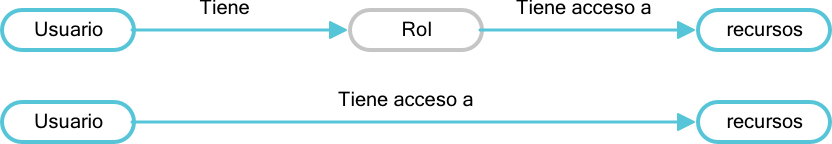
\includegraphics[width=1\textwidth]{firebase-auth}
  \caption{Autenticación basada en roles. (Fuente: Elaboración propia)}
\end{figure}

\subsubsection{Firebase Custom Claims}
Los roles de usuario son necesarios para identificar a los usuarios como administradores, gerentes o simplemente como clientes. Firebase Custom Claims permite establecer atributos de usuario simples directamente en el JWT del usuario (por ejemplo: \{ admin: true \}). Un JWT es un Json Web Token, es el objeto que contiene la información del usuario actual.
\vspace{0.8cm}

\lstinputlisting[label={firebase-auth}, style=ES6, caption=Fragmento para guardar crear y leer Firebase Custom Claims]{code/firebase-auth.js}

\subsection{Websockets con Socket.IO}
Si bien la base de datos Firebase Firestore proporciona una capa de conexión en tiempo real, es necesario introducir un nuevo método de comunicación permanente para notificar de eventos como lo son la presencia de usuarios activos y la visualización de las ordenes. Socket.IO permite la comunicación bidireccional entre el cliente y el servidor. Las comunicaciones bidireccionales se habilitan cuando un cliente tiene Socket.IO en el navegador, y un servidor también ha integrado el paquete. Si bien los datos se pueden enviar de varias formas, JSON es el más simple. Resume muchos tipos de transportes, incluidos \acrshort{ajax}  y \Glspl{websocket}, en una sola \acrshort{api}. Permite a los desarrolladores enviar y recibir datos sin preocuparse por la compatibilidad entre navegadores \cite{kelleher}.
\vspace{0.8cm}

En cualquier aplicación en tiempo real, mostrar múltiples usuarios en línea es muy importante, esta información debe actualizarse cuando un nuevo usuario se conecta o un usuario en línea se desconecta.
\vspace{0.8cm}

\begin{figure}[H]
  \centering
  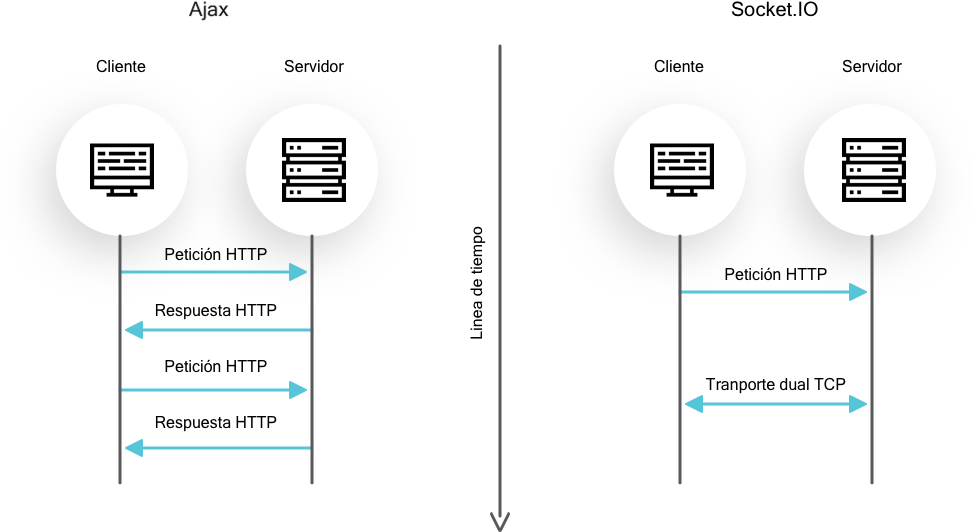
\includegraphics[width=1\textwidth]{websocket}
  \caption{Comparación de transporte por sondeo (Ajax) y Websockets (Socket.IO).}
\end{figure}

\lstinputlisting[style=ES6, caption=Fragmento de configuración de Socket.IO del sistema]{code/socket.js}
